\documentclass{article}
\usepackage[persian, group]{hw}

\geometry{
 a4paper,
 total={5in,7in}
 }
 
\title{گزارش نهایی}
\semester{نیم‌سال دوم ۰۰-۰۱}
\course{آز سخت‌افزار - گروه ۳}
\teacher{دکتر اجلالی}

\addauth{علی حاتمی تاجیک}{a.hatam008@gmail.com}{98101385}
\addauth{امیرمحمد عیسی‌زاده}{amirmohammadisazadeh@gmail.com}{98106807}
\addauth{*محمدحسین قیصریه}{mgheysariyeh@gmail.com}{97106238}

\usepackage{xcolor}

\definecolor{codegreen}{rgb}{0,0.6,0}
\definecolor{codegray}{rgb}{0.5,0.5,0.5}
\definecolor{codepurple}{rgb}{0.58,0,0.82}
\definecolor{backcolour}{rgb}{0.95,0.95,0.92}

\lstdefinestyle{mystyle}{
    backgroundcolor=\color{backcolour},   
    commentstyle=\color{codegreen},
    keywordstyle=\color{magenta},
    numberstyle=\tiny\color{codegray},
    stringstyle=\color{codepurple},
    basicstyle=\ttfamily\footnotesize,
    breakatwhitespace=false,         
    breaklines=true,                 
    captionpos=b,                    
    keepspaces=true,                 
    numbers=left,                    
    numbersep=5pt,                  
    showspaces=false,                
    showstringspaces=false,
    showtabs=false,                  
    tabsize=2
}

\lstset{style=mystyle}

\begin{document}

\heading
\header
\allowdisplaybreaks

\section{چکیده}

با گسترش تجهیزات کامپیوتری در سراسر جهان و افزایش کارایی و عملکرد آنها، زندگی بشر در ابعاد مختلف دچار تغییر و بهبود شده است. هوشمند سازی تجهیزات پیرامون از یک طرف و از طرف دیگر سادگی کار با تجهیزات زمینه جذاب و پرکابردی است که اخیرا بسیار مورد توجه قرار گرفته است. در واقع مسئله مورد نظر برگرفته از یک مشکل واقعی که انجام راحت تر دستورات کاربر با کامپیوتر است. در این پروژه ما سعی کردیم که هوشمند سازی ماوس را انجام دهیم و سامانه ای طراحی کنیم که بر اساس حرکات دست، دستورات کاربر را اجرا کند. علاوه بر اجرای دستورات عادی، به کاربر این امکان داده میشود که دستورات خاص تری را با حرکات تعریف شده دست انجام دهد.
\footnote{کد‌ها، گزارشات و باقی‌ فایل‌های مورد نیاز از طریق مخزن گیت‌هاب گروه که از طریق این 
\href{https://github.com/Sharif-University-ESRLab/project-team-3}{\textcolor{cyan}{لینک}}
قابل بارگیری‌ است.
همینطور فیلم مربوط به این پروژه بر روی
\href{https://www.aparat.com/v/ymRzw}{\color{cyan}{آپارات}}
قابل دسترسی است.
}

\vspace{0.5cm}

کلیدواژه ها: کنترل تصویری، ماوس تصویری، پردازش تصویر

\pagebreak
\tableofcontents
\pagebreak

\section{مقدمه}
در این فصل به طور خلاصه در مورد انگیزه اصلی پروژه و اهمیتش در زندگی روزمره صحبت خواهد شد.

\subsection{تعریف مسئله}
پردازش تصویر و فهمیدن فرمان انسان با پردازش حرکات آن از جانب کامپیوتر در دهه های اخیر مورد توجه بسیاری قرار گرفته است. اینکار میتواند فواید گوناگونی داشته باشد. اول اینکه با هوشمند سازی فهم دستورات، میتوانیم در وقت صرفه جویی کنیم و تجربه راحت تر و لذت بخش تری را برای کاربر ایجاد کنیم. در واقع سختی کار با ماوس فیزیکی، مسئله ای اجتناب ناپذیر است. بنابراین با حذف این آپشن، ماوس های تصویری جایگزین میشوند. این کار به کمک پردازش تصویر گرفته شده از دست کاربر که مکان و جابجایی هاي آن به حرکت نشانگر موشواره و عملیات هاي مربوط به آن منجر می شود. در کنار این تعدادي حالات قابل تعیین براي کاربر براي روانتر شدن داشته رابط کاربري وجود داشته باشد. در این پروژه نیازي به ماژول شدت صوت نیست و تمام حالت ها به وسیله پردازش تصویر قابل دستیابی هستند. 

\subsection{اهمیت مسئله}
این نکته شناخته شده است که کارکرد آسان تر وسایل جانبی می تواند علاوه بر تجربه مناسب کاربر، به دلیل راحتی استفاده، اثرات مثبت ذهنی و روانی نیز روی کاربر بگذارد. بدین جهت انسان از مدت ها قبل اقدام به استفاده از وسایل آسان تر به مرور زمان(مثل صفحات لمسی و ...) کرد؛ در دنیای امروزی ممکن است به دلیل کارهای زیاد و همزمان، رسیدگی به آنها برای کاربر دشوار باشد. بنابراین هر روشی که بتواند برای دادن راحت تر فرمان به رایانه به کاربر کمک بکند، اهمیت بالایی دارد. به طور خاص این پروژه می تواند به انجام دستورات توسط دست و با استفاده از پردازش تصویر کمک کند. استفاده زیاد از وسایل جانبی مانند ماوس، در درازمدت میتواند آسیب های فیزیکی به انسان بزند که مشکلات فراوانی از قبیل گرفتگی مچ دست، اذیت شدن انگشتان و ... را در پی دارد.

از سوی دیگر اگر به بعد های صنعتی بپردازیم، متوجه خواهیم بود که مسئله کمبود راهکار مناسب برای ارتباط با رایانه، مسئله بسیار جدی در شرکت های الکترونیکی است.

نکته دارای اهمیت این است که سال های زیادی است که شرکت های بزرگ به سمت ایده های جدید برای کار با وسایل الکترونیکی رفته اند، به عنوان مثال لمسی کردن صفحات گوشی ها و امروزه لمسی کردن صفحات بعضی از لپ تاپ ها، ولی مسئله این است که لمسی کردن لپتاپ ها از جهت هایی، کاری است که فلسفه درستی ندارد، چون قدرت پردازش و برق و ... برای جایی دارد مصرف میشود که نیاز کاربر نیست، به عبارتی کاربر اگر میخواست که فرمان هایش با لمس مانیتور اتفاق بیافتد که تلفن های همراه نیاز او را برطرف می‌کردند، نیاز اصلی کاربر این است که بتواند با ابزار های ساده کننده ای کار کند که حس استفاده از رایانه و نه تلفن همراه را به او القا کند. علاوه بر تمام دلایلی که آوردیم، لمس مانیتور کاری سخت است، چون ابعاد صفحه بزرگ است که موجب خستگی کاربر میشود.

\subsection{راهکار پیشنهادی}
در این پروژه هدف داریم راهکاری برای دادن فرمان های کاربر به رایانه با صرف انرژی کم ارائه دهیم، همچنین این امکان را برای کاربر فراهم سازیم تا با راحت تر شدن کار، زمان کمتری را صرف کند. در این قسمت راه حل پیشنهادی را به طور کلی مطرح می کنیم. توجه داشته باشید به طور کلی هرچقدر ما شناخت دقیق تری از نیاز کاربر داشته باشیم، آسان سازی ارتباط با رایانه به نحوه مطلوب تری صورت می گیرد. ما ابزاری را طراحی کردیم که کاربر با صرف انرژی بسیار کم، در همان جایی که هست، با استفاده از نوک انگشتانش، از راه دور دستوراتش را به رایانه بدهد. راه حل پیشنهادی ما بدین صورت است که با قراردادن یک دوربین در کنار نمایشگر، از حرکات کاربر فیلم برداری شود. سپس برای کم کردن بار پردازشی از روی پردازنده رایانه، از یک برد \lr{Raspberry Pi 3B+} استفاده شده است که تصاویر گرفته شده توسط دوربین، به آن داده می‌شود. سپس تحلیل ها برروی پردازش گر جانبی انجام میشود، و ساختار دست کاربر و حرکات آن بررسی می‌شود. در نهایت تحلیل های انجام شده در قالب دستوراتی به رایانه فرستاده می‌شود. این کار باعث قدرت استقلال از سیستم عامل می‌شود که بسیار بهتر از حالتی است که نیاز داریم پردازش ها بر روی رایانه انجام گیرد.
در نهایت پردازش های انجام شده بر روی پردازنده جانبی، با استفاده از کابل سریال، به رایانه فرستاده می‌شود و رایانه آن دستورات را تبدیل به دستورات \lr{IO} می‌کند.

\subsection{ساختار گزارش}
دراین گزارش سعی شده است که ابتدا نیاز مندی های سخت افزاری بررسی شود. بنابراین درفصل بعدی ابتدا به بررسی ماژول های سخت افزاری و انتظاری که از آنها داریم پرداخته می شود. سپس در فصل سوم به بررسی مشخصات ماژول های سخت افزاری انتخابی می پردازیم. در ادامه وارد نکات پیاده سازی پروژه می شویم. در فصل چهارم هم به آنالیز کد نرم افزاری پیاده سازی شده می پردازیم. در فصل آخر هم یک جمع بندی کلی پروژه داریم و مسائلی که در ادامه باید به آنها فکر شود، می پردازیم.


\section{مشخصات محصول}
مشخصات محصول همانگونه که در ورق داده \footnote{\lr{Datasheet}} آن آمده است در جدول \ref{spec} درج شده است.

% Please add the following required packages to your document preamble:
% \usepackage[table,xcdraw]{xcolor}
% If you use beamer only pass "xcolor=table" option, i.e. \documentclass[xcolor=table]{beamer}

\begin{table}[]
\begin{latin}
\begin{tabular}{|p{0.25\linewidth}|p{0.65\linewidth}|}
\hline
\rowcolor[HTML]{A5A5A5} 
 &
   \\ \hline
\rowcolor[HTML]{EDEDED} 
Size &
  100mm x 70mm x 34 mm (35.5mm camera top included) \\ \hline
Weight &
  25gr (packaging) + 43gr (processor) + 3g (camera)   = 71gr \\ \hline
\rowcolor[HTML]{EDEDED} 
Power Supply &
  AC 5V 2.5A via Micro USB connector (power supply is   not included) \\ \hline
Data   Connection &
  USB 2.0 (packaged with USB 2/3 hybrid   cable, but can be used with any certified USB standard cables with the   Hi-Speed USB 2.0 logo featured on the packaging) \\ \hline
\rowcolor[HTML]{EDEDED} 
Mounting &
  Should be placed on the desk with camera facing the   ceiling and the triangle on the top of the packaging showing "Up"   according to you (your hand) \\ \hline
Interaction   Zone &
  Minimum 30cm – Maximum 60cm distance from camera (depth) - 19cm boundary from camera at 30cm distance\\ \hline
\rowcolor[HTML]{EDEDED} 
Camera &
  One camera with OVA5647 sensor \\ \hline
Camera   Interface &
  Experimental Universal Video Class (UVC)   release provides access to low-level controls such as LED brightness, gamma,   exposure, gain, resolution, etc.; examples in C, Python, and Matlab, as well   as OpenCV binding \\ \hline
\rowcolor[HTML]{EDEDED} 
LED &
  At top right corner of the camera there is one LED   which is boot indicator. Whenever the LED is lightened up constantly, the device   is up and ready to use. \\ \hline
Construction &
  PLA and Acrylic \\ \hline
\rowcolor[HTML]{EDEDED} 
Ambient Operating Temperature &
  0 to 45 °C (RPi 3 Operating Temperature) \\ \hline
CPU   Temperature at Full Load (Ambient Temperature of 33 °C) &
  Min:   54 °C – Max: 72 °C – Average: 67.8 \\ \hline
\rowcolor[HTML]{EDEDED} 
FPS (Frame Per Second) &
  (Camera Capture) 32 FPS - (Capture and Run ML Model) Min: 1.5 – Max: 4.8 –   Average: 3.8 \\ \hline
Boot   Time &
  (Approximately) 51secs \\ \hline
\rowcolor[HTML]{EDEDED} 
Latency &
  (Approximately) 2 – 5 secs \\ \hline
Minimum   System Requirements &
  Windows 7, 8, 8.1, 10, 11 – MacOS X 10.7 – Linux   distros with GNU Gnome Desktop. \\ \hline
\end{tabular}
\end{latin}
\caption{مشخصات محصول}
\label{spec}
\end{table}


\section{سخت افزار مورد نیاز}
\subsection{واحد پردازشی}
برای واحد پردازشی از برد \lr{Raspberry Pi 3B+} استفاده شده است. \cite{pi} (شکل \ref{RPi3})
 
\begin{figure}
	\centering
	\includegraphics[scale=0.09]{./graphics/rpi3b.jpg}
	\caption{برد رزبری‌پای}
	\label{RPi3}
\end{figure}

\lr{Raspberry Pi 3} مجهز به یک پردازنده چهار هسته ای \lr{64} بیتی \lr{Broadcom BCM2837 ARM Cortex-A53 SoC} است که با فرکانس 1.2 گیگاهرتز کار می کند، که آن را حدود 50 درصد قدرتمندتر از \lr{Pi 2} می کند. این بدان معناست که \lr{Raspberry Pi 3} جدید می تواند برای برنامه های آفیس و مرور وب.

نوآوری بزرگ در این نسخه سوم بدون شک اضافه شدن تراشه \lr{WiFi} و بلوتوث کم انرژی است. این نه تنها باعث صرفه جویی در فضا می شود (دیگر نیازی به اتصال دانگل های \lr{WiFi} و بلوتوث ندارید)، بلکه پورت های \lr{USB} بیشتری را برای اتصال دستگاه های دیگر آزاد می کند.

با افزودن این دو ویژگی، \lr{Raspberry Pi} روشن کرده است که این نسخه جدید برای اینترنت اشیا (\lr{IoT}) و اتوماسیون خانگی طراحی شده است. \lr{Raspberry Pi 3} همچنین با \lr{Windows 10 IoT Core }سازگار است، سیستم عاملی که برای ایجاد و توسعه برنامه های کاربردی برای اتوماسیون خانگی، روباتیک و اشیاء متصل طراحی شده است.

برد \lr{Raspberry Pi 3} به اندازه \lr{Raspberry Pi 2} است و کانکتور و پیکربندی اجزا تقریباً یکسانی دارد. تنها چیزی که تغییر کرده است موقعیت \lr{LED} ها است که به سمت دیگر کارت \lr{SD} منتقل شده اند تا فضایی برای آنتن \lr{WiFi} ایجاد کنند. همه کانکتورها در یک مکان قرار دارند و عملکردهای یکسانی دارند. بنابراین می توان از لوازم جانبی \lr{Pi 2} و \lr{B+} خود با \lr{RasPi 3} نیز استفاده کرد.

مشخصه‌های سخت‌افزاری این برد به صورت زیر است:
\begin{latin}
\begin{itemize}
	\item Quad Core 1.2GHz Broadcom BCM2837 64bit CPU
	\item 1GB RAM
	\item BCM43438 wireless LAN and Bluetooth Low Energy (BLE) on board
	\item 100 Base Ethernet
	\item 40-pin extended GPIO
	\item 4 USB 2 ports
	\item 4 Pole stereo output and composite video port
	\item Full size HDMI
	\item CSI camera port for connecting a Raspberry Pi camera
	\item DSI display port for connecting a Raspberry Pi touchscreen display
	\item Micro SD port for loading your operating system and storing data
	\item Upgraded switched Micro USB power source up to 2.5A
\end{itemize}
\end{latin}

\subsection{تصویر‌برداری}
برای بخش تصویر‌برداری که به نوعی آشیل این پروژه به حساب می‌آید از ماژول دوربین رسپبری پای 
\lr{(5MP, 1080p, v1.3)}
استفاده شده است. (شکل \ref{cam}) 

\begin{figure}
	\centering
	\includegraphics[scale=0.3]{./graphics/cam.jpg}
	\caption{دوربین \lr{OVA5647}}
	\label{cam}
\end{figure}

دوربین برد رسپبری پای با استفاده از کانکتور \lr{CSI} مستقیما به برد رسپبری پای متصل می شود. این دوربین توانایی تصویر برداری با وضوح 5 مگاپیکسل و ضبط ویدیو با کیفیت \lr{1080p HD} را دارد. این ماژول با طراحی سفارشی خود توسط بنیاد رسپبری پای در انگلستان ساخته شده و دارای سنسوری با فوکوس ثابت و رزولوشن \lr{2592×1944} است. این ماژول از طریق کابل ریبون 15 پینه به رسپبری پای متصل می شود و از رابط سریال دوربین که مختص اتصال دوربین ها ساخته شده ،  استفاده می کند. \lr{CSI} قابلیت انتقال نرخ بسیار بالایی از داده ها را دارد.

برد این ماژول کوچک و به اندازه ی \lr{20x25x9} میلیمتر  و وزن آن تنها 3 گرم است، به همین دلیل برای استفاده در پروژه هایی که وزن و ابعاد قطعات اهمیت بالایی دارند، گزینه ی بسیار مناسبی است. سنسور این ماژول دارای رزولوشن 5 مگاپیکسل و لنز آن دارای فوکوس ثابت است که آن را قادر به دریافت و ارائه ی تصاویر استاتیک با کیفیت \lr{2592x1944} پیکسل و همچنین قابلیت پشتیبانی از  \lr{1080p @ 30fps, 720p @ 60fps} و  \lr{640x480p 60/90} برای ضبط ویدیو می سازد.

این ماژول تا آخرین نسخه ی \lr{Raspbian} که سیستم عامل مورد استفاده در رسپبری پای است را پشتیبانی می کند.

مشخصه‌های این دوربین به شرح زیر است:
\begin{itemize}
	\item سازگاری کامل با مدل ها \lr{A} و \lr{B} رسپبری پای
	\item ماژول دوربین \lr{5MP Omnivision 5647}
	\item رزولوشن عکس \lr{2592x1944}
	\item پشتیبانی از  \lr{1080p @ 30fps}, \lr{720p @ 60fps} و  \lr{640x480p 60/90} برای ضبط ویدیو
	\item رابط سریال دوربین-15 پین  \lr{MIPI} - تغذیه مستقیم از برد رسپبری پای
	\item ابعاد :  \lr{20 x 25 x 9} میلیمتر
	\item وزن : 3 گرم
\end{itemize}		

\subsection{ارتباطات}
برای ارتباط بین برد رسپبری‌پای و رایانه مقصد از ماژول سریال \lr{TTL} استفاده
شده است که به صورت کابل درامده است و استفاده راحت‌تری و شکیل‌تری نسبت به ماژول خام دارد.
(شکل \ref{usb})

\begin{figure}
	\centering
	\includegraphics[scale=0.3]{./graphics/usb.jpg}
	\caption{ماژول \lr{TTL-USB}}
	\label{usb}
\end{figure}

 مشخصات فنی این کابل:
 \begin{itemize}
 	\item بر اساس ماژول \lr{PL2303HX}
 	\item شاخصه‌ سیم‌ها نیز به صورت زیر است:
 	\begin{itemize}[*]
 		\item قرمز : پاور
 		\item سیاه : زمین
 		\item سفید : \lr{RX} در پورت \lr{USB}
 		\item سبز :  \lr{TX} در پورت \lr{USB}
 	\end{itemize}
 \end{itemize}

\subsection{بسته‌بندی محصول}
برای بسته‌بندی این محصول برای استفاده حداکثری از فضا و زیبایی و شکیل بودن محصول نهایی تصمیم
گرفته شده است تا بسته‌بندی محصول توسط پرینترهای سه‌بعدی تهیه شوند. این شکل بسته‌بندی به این دلیل که انعطاف‌پذیری زیادی برای طراح دارد می‌تواند طرح‌های زیبا و چشم‌نوازی را خلق کند و باعث
افزایش فروش محصول به خاطر ظاهر زیبا شود. البته این روش (پرینتر سه‌بعدی) برای تعداد بالای
محصول پاسخگو نیست و در صورتی که تولید انبوه صورت بگیرد با استفاده از قالب، و پالیش نهایی
می‌توان با سرعت بالاتری به همان نتیجه رسید با این هزینه که تهیه تجهیزات مورد نیاز برای این
کار بسیار بالاتر خواهد بود. در اصل پرینترهای سه‌بعدی اکثرا برای طرح اولیه استفاده می‌شوند. شکل \ref{case} نشان‌دهنده طرح‌های اولیه برای بسته‌بندی است. البته این طرح‌ها با احتمال خوبی دستخوش تغییر خواهد شد.

طراحی بسته‌بندی به گونه‌ایست که کمترین‌ فضای ممکن را اشغال کند. همچنین تهویه مناسب برای پردازنده
نیز در نظر گرفته شده است و شیار‌هایی در رو و زیر جعبه تعبیه شده‌اند. 
نام دستگاه روی جعبه هک می‌شود و همچنین یک مثلث که نمایانگر بالای محصول است نیز وجود دارد. 
طبق این طراحی کابل تغذیه را کاربر باید به صورت جداگانه به محصول متصل کند اما کابل
انتقال اطلاعات به طول ۸۰ سانتی‌متر به صورت غیرقابل جدا‌شدن به دستگاه متصل می‌شود.
بر روی قسمت پایینی چهار پایه برای ساپورت‌ کردن برد رزبری‌پای در جای خود قرار دارد. همچنین
بر روی در چهار پایه برای نگه‌داشتن دوربین پیش‌بینی شده است.
درب محصول به صورت \lr{Snap Fit} طراحی شده است و به صورت یک مکانیزم کلیکی بر روی آن محکم می‌شود.
البته بست در نظر گرفته شده به این منظور طراحی شده است که تا مدت زمان زیادی درب را بسته نگه‌دارد
و مناسب برای باز و بسته شدن‌های پیاپی نیست! در گوشه سمت راست-بالای سوراخ دوربین یک سوراخ وجود دارد
که نمایانگر روشن بودن دستگاه است. زمانی که این \lr{LED} به صورت ممتد روشن باشد
نشان دهنده این موضوع است که دستگاه به صورت کامل بوت شده است.


طراحی بدنه به وسیله نرم‌افزار \lr{Fusion 360} انجام شده است و چاپ پروتوتایپ اولیه آن به وسیله پرینتر \lr{Ultimaker} و به کمک نرم‌افزار مخصوص این شرکت - \lr{Cura} - انجام گرفته است.

\begin{figure}
	\centering
	
	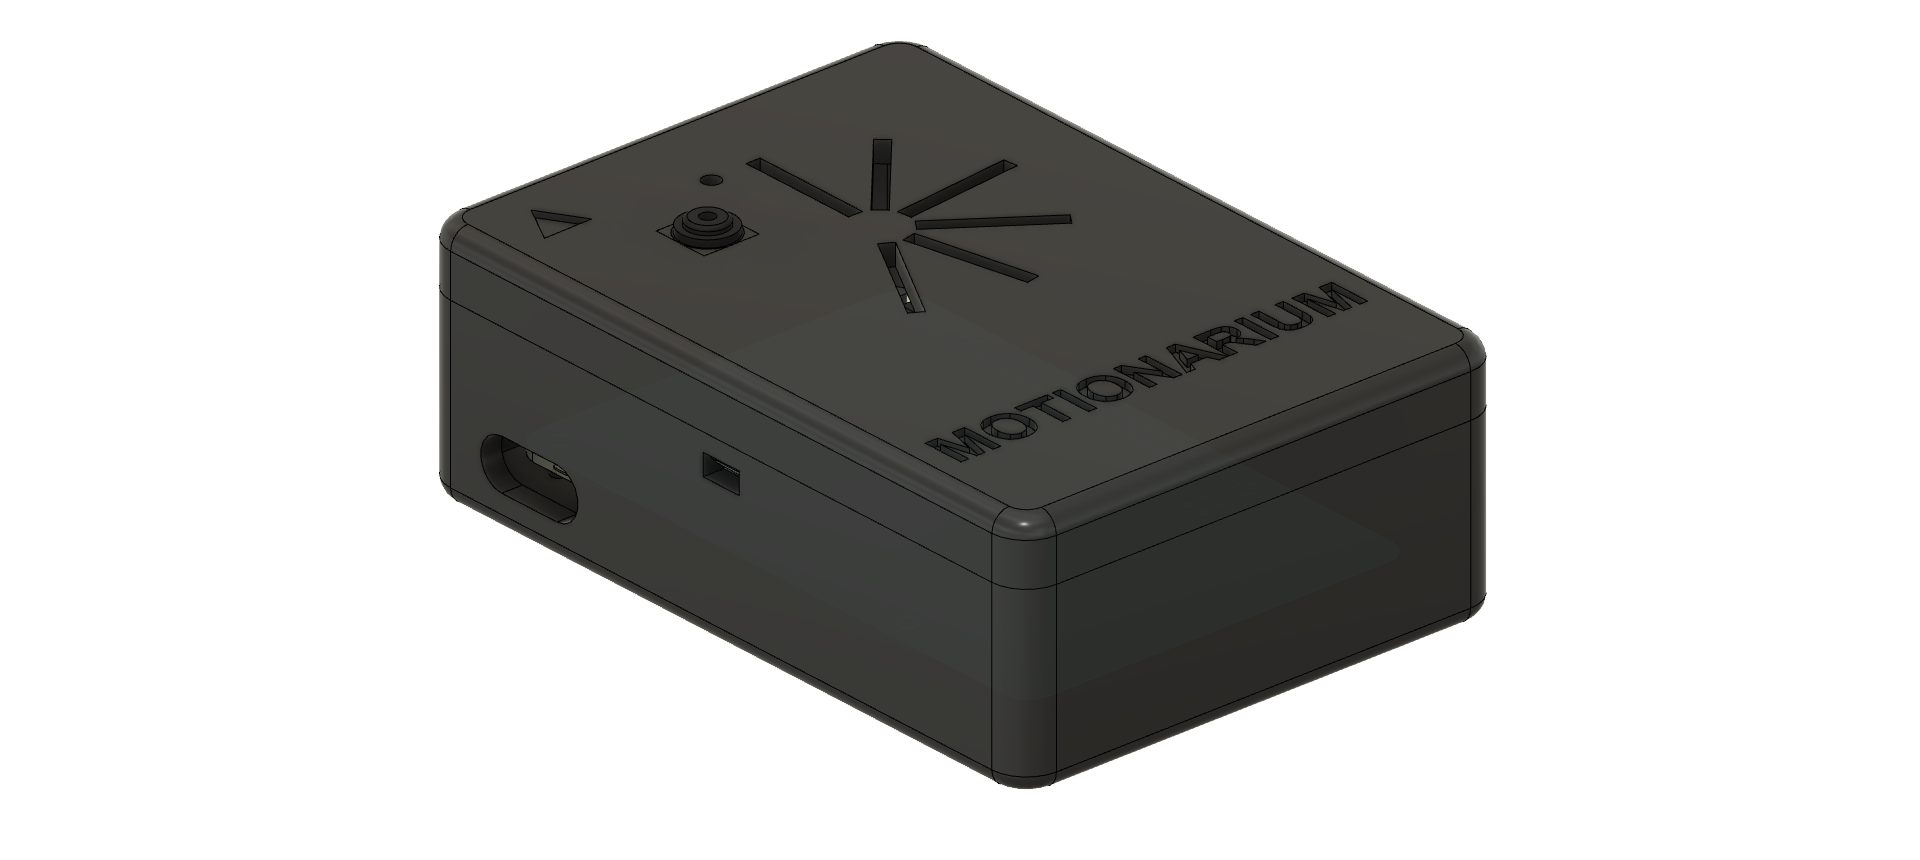
\includegraphics[width=7cm]{./graphics/main}
	
	\includegraphics[width=5cm]{./graphics/bottom}
	\includegraphics[width=5cm]{./graphics/bottom2}
	
	\includegraphics[width=5cm]{./graphics/bottom3}
	
	\includegraphics[width=5cm]{./graphics/top}
	\includegraphics[width=5cm]{./graphics/top2}
	
	\caption{بسته‌بندی محصول}
	\label{case}
\end{figure}

\section{نحوه پیکر‌بندی سخت‌افزار}
\subsection{دیاگرام سیستم}
در شکل \ref{chart} دیاگرام کلی طرز کار سیستم‌ آمده است. روند کلی کار به این صورت است که
ابتدا تصویر از محیط اطراف گرفته \footnote{\lr{Capture}} می‌شود. سپس با استفاده از رابط \lr{CSI} به واحد پردازشی منتقل می‌شود. زمانی که تصویر در واحد پردازشی دریافت شد مدل هوش
مصنوعی که از قبل تمرین‌داده \footnote{\lr{train}} شده است روی تصویر پردازش انجام می‌دهد که
نتیجه آن تشخیص محل دست‌ها و نقاط عطف آن است. پس از آن، این نقاط عطف تفسیر می‌شوند و نتیجه با
استفاده از رابط سریال به رایانه مقصد منتقل می‌شود و از آنجا با استفاده از درایورش  تفسیر
نهایی و تبدیل به حرکات موشواره روی آن صورت می‌گیرد.

\begin{figure}
	\centering
	\includegraphics[scale=0.5]{./graphics/chart.jpg}
	\caption{دیاگرام سیستم}
	\label{chart}
\end{figure}


\subsection{پیکربندی}
پیکربندی نرم‌افزاری شامل دو مورد است. اول اتصال دوربین به برد که با استفاده از یک کابل صاف
\footnote{\lr{flat}} انجام می‌گیرد.  (شکل \ref{cam-cable})

\begin{figure}
	\centering
	\includegraphics[scale=0.4]{./graphics/cam-cable.jpg}
	\caption{اتصال دوربین رزبری‌پای}
	\label{cam-cable}
\end{figure}

پیکربندی ماژول \lr{TTL} نیز به این صورت انجام میگیرد که پایه‌های \lr{TX, RX} به صورت برعکس به مشابهشان در رزبری وصل می‌شوند و همچنین پایه‌ زمین \footnote{\lr{GND, Ground}} به زمین برد
متصل می‌شود تا زمین‌ها مشترک باشند. البته بنا بر این بود تا سیم قدرت نیز به برد متصل شود و
قدرت مورد نیاز برد از طریق درگاه \lr{USB} لپ‌تاپ تامین شود اما با توجه به معیوب بودن ماژول
خریداری شده و انتقال قدرت نامناسب و ناامن و غیرقابل اعتماد \footnote{\lr{unreliable}}
تصمیمم بر این شد که توان مورد نیاز برد به صورت مستقیم از طریق منبع توان تامین شود.
پیکربندی این ماژول در شکل \ref{ttl-conf} قابل مشاهده است.

\begin{figure}
	\centering
	\includegraphics[scale=0.4]{./graphics/ttl-conf.png}
	\caption{اتصال ماژول سریال}
	\label{ttl-conf}
\end{figure}

\section{نحوه پیاده‌سازی نرم افزاری}
در ابتدا از تصمیم بر استفاده از ماژول های نوشته شده و آماده بود ولی بعد از تست کردن برخی از آن‌ها و کارکرد نامطلوبشان، تصمیم گرفتیم که این ماژول ها را خودمان طراحی کنیم.
 
کد های پروژه شامل سه بخش اصلی است که هر کدام به تفصیل توضیح داده خواهند شد. برای پیاده سازی نرم افزاری پروژه نیاز داریم تا در ابتدا ماژولی دست ما را تشخیص دهد، سپس حرکات دست تعبیر شوند، سپس این تعابیر به صورت دستوری خلاصه مانند کلیک راست، یا حرکت نشانگر یا ... درآورده شوند. سپس این تعابیر از پردازنده جانبی به رایانه فرستاده شوند، سپس با توجه به نوع دستور فرستاده شده، تعبیر \lr{IO}  معلوم شود و در نهایت این تعبیر به صورت یک دستور \lr{IO} انجام شود.

تمامی کد های این پروژه با استفاده از زبان برنامه نویسی \lr{python} ورژن 3 زده شده است. بخش تشخیص دست و انگشتان و ... در فایل
\verb~handdetector.py~
 آورده شده است. بخش تعبیر حرکات و تبدیل یک سری حرکات مشخص به دستور خاص در فایل 
 \verb~handler.py~
  آورده شده است.

\subsection{ماژول \lr{handdetector.py}}
این ماژول که بخش اصلی و هسته این پروژه است وظیفه تشخیص دست، پیدا کردن مکان نقاط از پیش تعیین شده، پیدا کردن فاصله بین دو نقطه و پیدا کردن اینکه کدام انگشت ها در حال حاضر بالا هستند را دارد.
نقطه اصلی این ماژول، کتابخانه \lr{mediapipe}  است که کار های پردازش تصویر را انجام می‌دهد. این کتابخانه توسط گوگل توسعه یافته. برای این منظور یک کلاس \lr{HandDetector} تعریف شده و این توابع در آن پیاده سازی شده‌اند.
کتابخانه \lr{mediapipe} امکانات فراوانی از جمله تشخیص دست، تشخیص چهره، تشخیص محدوده مو و ... را دارد. کارکرد این کتابخانه در این پروژه قسمت تشخیص دست آن یا همان \lr{hand detection} است. استفاده ما از این کتابخانه در این پروژه پیدا کردن مکان یک سری نقاط مشخص روی دست است و سایر کار ها را از روی مکان این نقاط انجام می‌دهیم.

\begin{figure}
	\centering
	\includegraphics[scale=0.22]{./graphics/hand_landmarks.png}
	\caption{نقاط عطف (\lr{Landmark})}
	\label{landmark}
\end{figure}

شکل \ref{landmark} همان 20 نقطه مد نظر است، می‌توان گفت که مهم ترین بین این نقاط، نقطه هشت یا همان نوک انگشت اشاره است. این نقطه معلوم کننده جای نشانگر ماوس است. در ادامه می‌بینید که مثلا از فاصله این نقطه با دست، می‌توان فهمید که انگشت اشاره بالا است یا خیر.
\cite{medipipe}

برای نشان دادن محدوده دست و جای انگشتان و ... بر روی نمایشگر از کتابخانه \lr{openCV} استفاده می‌شود. تصاویر ضبط شده با کتابخانه \lr{mediapipe} توسط این کتابخانه نمایش داده می‌شوند. 
\cite{cv2}

هم‌اکنون به توابع این فایل می‌پردازیم و کارکرد آنها را با هم بررسی می‌کنیم.

\begin{latin}
\begin{lstlisting}[language=python]
def findHands(self, img, draw=False):
    imgRGB = cv2.cvtColor(img, cv2.COLOR_BGR2RGB)
    self.results = self.hands.process(imgRGB)

    if draw:
        if self.results.multi_hand_landmarks:
            for handLms in self.results.multi_hand_landmarks:
                self.mp_drawing.draw_landmarks(img, handLms,
                                  self.mp_hands.HAND_CONNECTIONS)
\end{lstlisting}
\end{latin}

تابع \lr{findHands}:
این تابع برای پیدا کردن دست(ها) استفاده می‌شود، به طوری تصویر گرفته شده از وبکم را دریافت می‌کند سپس آن را به صورت یک عکس \lr{cv2} در می‌آورد و در نهایت این عکس را به تابع \lr{mediapipe.hands.process} می‌دهد، که نتیجه آن آبجکت های دست ها است که در متغیر \lr{hands} ذخیره می‌شوند و اگر مقدار متغیر \lr{draw} برابر با \lr{True} باشد، جای دست و ... را روی تصویر می‌کشد.

\begin{latin}
\begin{lstlisting}[language=python]
def findPosition(self, img, handNo=0, draw=False):
    xList = []
    yList = []
    bbox = []
    self.lmList = []
    if self.results.multi_hand_landmarks:
        myHand = self.results.multi_hand_landmarks[handNo]
        for id, lm in enumerate(myHand.landmark):
            # print(id, lm)
            h, w, c = img.shape
            cx, cy = int(lm.x * w), int(lm.y * h)
            xList.append(cx)
            yList.append(cy)
            # print(id, cx, cy)
            self.lmList.append([id, cx, cy, lm.z])
            if draw:
                cv2.circle(img, (cx, cy), 5, (255, 0, 255), cv2.FILLED)

        xmin, xmax = min(xList), max(xList)
        ymin, ymax = min(yList), max(yList)
        bbox = xmin, ymin, xmax, ymax

        if draw:
            cv2.rectangle(img, (xmin - 20, ymin - 20), (xmax + 20, ymax + 20),
                            (0, 255, 0), 2)

    return self.lmList, bbox
\end{lstlisting}
\end{latin}

این تابع برای ذخیره سازی جایگاه نقطه های مورد نظر است. به این شکل که این نقاط را در متغیر های \lr{XList} و \lr{YList} که لیست هستند می‌ریزد. و در نهایت اگر متغیر \lr{draw} برابر با \lr{True} باشد دور دست یک مستطیل می‌کشد یا به عبارتی محدوده آن را معلوم می‌کند. محدوده دست به این شکل است که پایین ترین و بالاترین  \lr{x }ها و \lr{y} ها را ذخیره می‌کند و از هر ظرف 20 پیکسل حاشیه می‌دهد تا به خوبی معلوم شود.

\begin{latin}
\begin{lstlisting}[language=python]
def findDistance(self, p1, p2, img, draw=False, r=15, t=3):
    x1, y1 = self.lmList[p1][1:3]
    x2, y2 = self.lmList[p2][1:3]
    cx, cy = (x1 + x2) // 2, (y1 + y2) // 2

    if draw:
        cv2.line(img, (x1, y1), (x2, y2), (255, 0, 255), t)
        cv2.circle(img, (x1, y1), r, (255, 0, 255), cv2.FILLED)
        cv2.circle(img, (x2, y2), r, (255, 0, 255), cv2.FILLED)
        cv2.circle(img, (cx, cy), r, (0, 0, 255), cv2.FILLED)
    length = math.hypot(x2 - x1, y2 - y1)

    return length, img, [x1, y1, x2, y2, cx, cy]
\end{lstlisting}
\end{latin}

این تابع فاصله بین دو نقطه عطف را در دست پیدا می‌کند (فاصله اقلیدسی) و اگر متغیر 
\lr{draw}
مقدار یک داشته باشد یک خط بین دو انگشت می‌کشد و بین آنرا با رنگ قرمز پر می‌کند که نشان‌دهنده این باشد که فاصله بین این دو انگشت اندازه گرفته شده است.

\subsection{ماژول \lr{handler.py}}
این ماژول که مسئول تعبیر حالت های دست و اطلاعات دریافت شده از ماژول \lr{handdetector.py} است، شامل یک حلقه \lr{while} بی‌نهایت است که در هر لحظه اطلاعات را تفسیر می‌کند و آنها را به دستو قابل فهم تبدیل می‌کند و آن را به صورت سریال برای رایانه ارسال می‌کند.

این ماژول به صورت یک سرویس روی برد رزبری‌پای پیکربندی شده است تا با هربار بوت شدن سیستم (اتصال به برق) به صورت خودکار اجرا شده و کارهای مربوط به خود را انجام دهد.

کتابخانه های اصلی این ماژول، کتابخانه های \lr{numpy} و \lr{serial} و ماژول \lr{handdetector} هستند. یکی از اتفاقات مهمی که در این ماژول رخ می‌دهد، ست کردن اندازه وبکم است، چون اندازه ای که دوربین می‌گیرد، \lr{2592x1944} پیکسل است که پردازش این مقدار پیکسل برای مدل هوش مصنوعی بسیار زمان بر است، پس اندازه تصویر را در ابتدا به \lr{320x240} پیکسل تغییر می‌دهیم. بقیه قسمت های این ماژول را برای تفهیم بهتر کارکرد آنها با شکل نمایش می‌دهیم.

در حلقه در هر لحظه تصویر خوانده می‌شود و سپس جای دست و انگشت ها به خصوص انگشت اشاره و انگشت وسط پیدا می‌شوند. سپس در تابع \lr{fingersUp} که در ماژول \lr{handdetector} پیاده سازی شد، انگشت هایی که بالا هستند شناسایی می‌شوند. شایان به ذکر است که متغیر \lr{fingers} یک لیست پنج تایی است که نمایانگر پنج تا انگشت است، اگر مقدار انگشتی یک بود یعنی آن انگشت بالا و اگر مقدارش صفر بود یعنی پایین است. حال با توجه به متغیر هایی که تا الان تعریف کردیم، چندین تفسیر برای عکس وجود دارد که به شرح زیر است:

\begin{itemize}
	\item حالت حرکت:
	این حالت زمانی رخ می‌دهد که فقط انگشت اشاره بالا باشد و انگشت وسط پایین باشد، در این صورت به حالت حرکت می‌رویم و در این حالت هر جا که نوک انگشت اشاره برود، به نقطه ای در صفحه 
	نمایشگر نگاشت می‌شود.
\begin{latin}
\begin{lstlisting}[language=python]
		# 4. Only Index Finger : Moving Mode
    		if fingers[1] == 1 and fingers[2] == 0:
        	# 7. Move Mouse
        	ser.write (b"v*%d*%d\n"%(x1,y1))
\end{lstlisting}
\end{latin}
	
	\item حالت کلیک دوتایی:
	این حالت زمانی است که هر دو انگشت اشاره و وسط بالا باشند، به این حالت می‌رویم. به این صورت که وقتی هر دو بالا می‌روند کار دیگری نمی‌توانیم بکنیم و به عبارتی نمی‌توانیم نشانگر را تکان دهیم، تا زمانی که یا از این حالت بیرون بیاییم یا اینکه دو تا انگشت را به هم نزدیک کنیم و اگر فاصله از 15 پیکسل کمتر شد، دابل کلیک انجام می‌شود.
	
\begin{latin}
\begin{lstlisting}[language=python]
if fingers == [0,1,1,0,0]:
    print('dclick-mode')
    # 9. Find distance between fingers
    length, img, lineInfo = detector.findDistance(8, 12, img)
    # 10. Click mouse if distance short
    if length < 15:
        if not dclicked:
            ser.write(b"d\n")
            dclicked = True
    else:
        dclicked = False
\end{lstlisting}	
\end{latin}
	\item حالت کلیک تکی:
	این حالت زمانی است که انگشت اشاره و دو انگشت وسط بالا باشند، سپس اگر فاصله انگشت اشاره و انگشت وسط کمتر از 15 پیکسل شد، چپ کلیک اتفاق می‌افتد و مقدار \lr{clicked} هم \lr{True} می‌شود و در غیر این صورت مقدار آن \lr{False} می‌شود.	
	
	
	\item حالت درگ‌اند‌دراپ:
	وقتی انگشت اشاره و انگشت شست با هم بالا باشند به حالت \lr{drag and drop} می‌رویم، به این صورت که اگر فاصله این دو انگشت از 15 پیکسل کمتر شود \lr{mousedown} یا همان \lr{drag} رخ می‌دهد و اگر در حالت \lr{drag} باشیم و فاصله بیشتر از 15 پیکسل شود، \lr{mouseup} یا همان \lr{drop} می‌کنیم و مقدار \lr{mouseDown} هم برابر با \lr{False} میگذاریم.
	
	\item حالت راست کلیک:
	این حالت زمانی اتفاق می‌افتد که انگشت اشاره و انگشت شست و انگشت وسط با هم بالا باشند. اگر فاصله انگشت اشاره و انگشت وسط کمتر از 15 پیکسل شود، راست کلیک اتفاق می‌افتد.
	
	\item حالت اسکرول:
	این حالت زمانی اتفاق می‌افتد که تمامی انگشت ها بجز شست بالا باشند به حالت اسکرول می‌رویم. حال اگر دستمان را بالا رویم، اسکرول پایین اتفاق می‌افتد و اگر دستمان را پایین ببریم، اسکرول بالا اتفاق می‌افتد(مثل صفحه تاچ لپ‌تاپ که وقتی به بالا دستمان را می‌بریم، صفحه پایین می‌آید و وقتی پایین می‌بریم، بالا می‌رود.)
	
\begin{latin}
\begin{lstlisting}[language=python]
if fingers == [0,1,1,1,1]:
    # scroll mode
    pos = y1
    if last_pos_scroll == -1:
        last_pos_scroll = pos
    else:
        if abs(last_pos_scroll - pos) > 10:
            clicks = int((last_pos_scroll - pos))
            ser.write (b"s*%d\n"%(clicks))
            last_pos_scroll = pos
\end{lstlisting}	
\end{latin}
	
	
	\item اسکرین‌شات:
	با باز کردن انگشت کوچک و انگشت شصت و بستن باقی انگشتان این حالت فعال می‌شود. برای جلوگیری از اسکرین شات گرفتن مداوم فاصله زمانی یک ثانیه‌ای بین هر دستور اسکرین شات قرار گرفته است.
	
\begin{latin}
\begin{lstlisting}[language=python]
if fingers == [1,0,0,0,1]:
    if time.time_ns() - last_ss > 1_000_000_000:
        last_ss = time.time_ns()
        ser.write (b"p\n")
\end{lstlisting}	
\end{latin}
	
\end{itemize}

\subsection{درایور}
درایور آن بخشی از از قسمت نرم‌افزاری است که در سمت رایانه مقصد اجرا می‌شود. در موضوعی که ما از آن استفاده می‌کنیم درایور ابتدا به رابط سریال محصول متصل می‌شود. سپس ارتباطی را با آن آغاز کرده و اگر ارتباط امکان پذیر باشد دستورات را از آن می‌خواند و عملیات‌های لازم را به سیستم‌عامل اعلام می‌ کند. 

درایور مورد استفاده ما از دو فرآیند \footnote{\lr{Process}} کلی تشکیل شده است:

\begin{itemize}
	\item \lr{Interpreter}: این بخش مربوط به گرفتن و خواندن دستورات و اعمال تغییرات لازم بر سیستم‌عامل است.
	در این قسمت پس از اینکه دستورات از سریال که توسط ویژوالایزر انتخاب شده است (توضیح در بعد) یک خط از دستورات را خواند ابتدا چک می‌کند که فرمت ارسالی دستور درست باشد و داده‌های اشتباهی فرستاده نشده‌باشد. سپس اگر فرمت دستور با فرمت دستوراتی که برای برنامه تعریف شده است هم‌خوانی داشته باشد، با توجه به نوع دستور (اولین بایتی که ارسال می‌شود) به صورت داینامیک تابع مربوط به آن انتخاب می‌شود و پارامترهایی (یک یا چند عدد صحیح) که با آن ارسال شده است به تابع پاس داده می‌شود تا عملیات‌های خود را انجام دهد.
	
	عملیات‌های انجام شده توسط کتابخانه
	\verb~pyautogui~ انجام می‌شود که امکان فرستادن دستورات موشواره و کیبورد را به سیستم‌عامل دارد البته برای اینکه بتوان از این کلیک‌ها و ... روی قسمت‌های امنتیتی ویندوز نیز استفاده کرد باید درایور به صورت \lr{Administrator} اجرا شود. \cite{gui-osk}
	
	خلاصه کدی که در این بخش اجرا می‌شود به شرح زیر است:
\begin{latin}
\begin{lstlisting}[language=python]
def get_command():
    # wait till a new command is received
    command = get_serial_line()
    if command:
        for pattern in patterns:
            # search in the patterns if the command exists or not
            x = re.search(pattern, command)
            if x:
                # seperate command and its parameters
                x = list(x.groups())
                return x[0], x[1:]
        return None, None
    else:
        # sleep to prevent busy waiting until a serial is connected
        time.sleep(0.5)
        return None, None


def interpret(command: str, params: list):
    # finds corresponding handler of the command and do the command
    globals()["do_"+command](params)

def start():
    global visualizer
    visualizer = Visualizer()
    visualizer.start()
    while True:
        try:
            # get command from serial
            command, params = get_command()
            if command:
                # interprate command
                interpret(command, params)
        except Exception as e:
            # log bad habits
            logger.log(3, str(e))
\end{lstlisting}	
\end{latin}

تابع \verb~interpret~ به این صورت کار می‌کند که از سیمبل‌هایی که به صورت جهانی در اسکریپت
تعریف شده است آن سمبلی که با
\verb~do_~
آغاز می‌شود و پایانش با نام کانمند ما است (توابع متناسب در فایل تعریف شده‌اند) را انتخاب و پاس دادن پارامترها اجرا کن.

لیست دستوراتی که درایور از آن پشتیبانی می‌کند نیز به صورت زیر است:
\begin{latin}
\begin{lstlisting}[language=python]
# patterns send from RPi
patterns = [
    "^(b)[*]([-]?\d+)[*]([-]?\d+)[*]([-]?\d+)[*]([-]?\d+)$",
    "^(v)[*]([-]?\d+)[*]([-]?\d+)$",
    "^(d)$",
    "^(md)$",
    "^(mu)$",
    "^(c)$",
    "^(r)$",
    "^(s)[*]([-]?\d+)$",
    "^p$"
]
\end{lstlisting}	
\end{latin}
	
	\item \lr{Visualizer}: این بخش مسئول نشان‌دادن تفاسیر برنامه از حرکات کاربر به صورت گرافیکی و فراهم کردن ساز و کاری برای انتخاب پورت دستگاه است که البته در حال حاضر ساختار گرافیکی ساده‌ای دارد. به خاطر طویل بودن کدهای مربوط به \lr{GUI}/ از آوردن آنها خودداری شده است اما کدها به صورت کامل کامنت‌گذاری شده‌اند. تصویری از این رابط کاربری در شکل \ref{gui}
	آمده است.
	این رابط کاربری در زمان اجرا در گوشه بالا سمت راست است و برای اینکه کاربر بتواند تمام محتوای صحفه را ببیند به صورت محو در صفحه ظاهر می‌شود که البته توسط کاربر قابل جابجایی است و با درگ اند دراپ در هر جای صفحه می‌تواند قرار بگیرد. این نمایشگر همیشه روی برنامه‌های دیگر قرار می‌گیرد و زیر صفحه دیگری نمی‌رود. برای بستن آن نیز کافی‌است تا با راست کلیک روی آن از منوی مربوط گزینه \lr{Exit}  انتخاب شود.
	
	دارای یک کادر قرمز‌رنگ است که نشان‌دهنده صفحه کاربر (با اندازه دوربین) است. مستطیل سیاه (که در شکل مشخص نیست) نشان‌دهنده حدود دست است و دایره آبی رنگ نشان‌دهنده نوک انگشت سبابه کاربر است. در بالاترین بخش آن نیز یک منوی کشویی \footnote{\lr{Drop Down Menu}}
قرار دارد که در هربار باز کردن این منو لیستی از پورت‌های سریال متصل به رایانه به کاربر
نمایش داده می‌شود که کاربر باید پورت مربوط به محصول را از بین آن انتخاب کند.

	\begin{figure}
		\centering
		\includegraphics[scale=0.5]{./graphics/driver.jpg}
		\caption{نمایی از ویژوالایزر درایور}
		\label{gui}
	\end{figure}
	
\end{itemize}

\section{پیکربندی سیستم}
در این بخش به پیکر‌بندی‌هایی لازم برای سیستم (هم برد و هم رایانه مقصد)‌ می‌پردازیم.

\subsection{پیکربندی رسبپری‌پای}
\subsubsection{نصب سیستم‌عامل ۶۴بیتی}
برای اینکه بتوانیم از کتابخانه مدیاپایپ بر روی بردهای رزبری پای استفاده کنیم باید این برد به صورت ویژه پیکربندی بشود چراکه این کتابخانه برای سیستم‌عامل‌های ۳۲ بیتی توسعه نیافته است و در صورت نیاز برای استفاده از آنها کاربر باید خود این کتابخانه را بسازد\footnote{\lr{Build}}.

برای ساختن این کتابخانه به ابزار \lr{Bazel} نیاز است که برای نصب آن روی برد‌های رزبری‌پای به حداقل ۱۶ گیگابایت حافظه نیاز است که با توجه به اینکه حافظه فعلی ما یک \lr{SD} ۸ گیگابایتی است این کار مقدور نبود و پس از چندین بار تلاش، به نتیجه‌ای نرسید.

برای همین باید یک سیستم‌عامل ۶۴ بیتی (که خوشبختانه چند ماهی ‌است برای بردهای رزبری‌پای توسعه‌ یافته است) استفاده کنیم. برای این کار باید تصویر \footnote{\lr{Image - iso file}} مربوط به این سیستم‌عامل روی \lr{SD} کارت نوشته شود که بهترین گزینه برای انجام این کار نرم‌افزار رسمی رسپبری‌پای یعنی \lr{Raspberry Pi Imager} است. پس از انتخاب نسخه ۶۴ بیتی و درایو مورد نظر، این نرم‌افزار سیستم‌عامل را از منابع معتبر دانلود کرده و آن را روی کارت حافظه تصویر می‌کند (شکل \ref{RPi Imager}).

همچنین این نرم‌افزار کانفیگ‌های لازم برای راه‌اندازی برد به صورت \lr{Headless} را نیز در اختیار ما قرار می‌دهد. این کار با استفاده از پیکربندی اتصال وای‌فای و فعال‌سازی سرویس \lr{SSH} امکان‌پذیر است.

\begin{figure}
	\centering
	\includegraphics[scale=0.5]{./graphics/rpiimager.jpg}
	\caption{\lr{Raspberry Pi Imager}}
	\label{RPi Imager}
\end{figure}

شکل \ref{64} نشان‌دهنده موفقیت‌آمیز بودن این عملیات است.

\begin{figure}
	\centering
	\includegraphics[scale=0.5]{./graphics/64.jpg}
	\caption{سیستم‌عامل ۶۴ بیتی}
	\label{64}
\end{figure}

\subsection{نصب‌کتابخانه‌های لازم}
پس از اینکه سیستم‌عامل به خوبی پیکربندی شد، باید کتابخانه‌هایی که سرویس تشخیص حرکات دست به آن نیاز دارد را نصب کرد. این کتابخانه‌ها به وسیله دستور
\verb~pip~
قابل نصب هستند:
\begin{latin}
    \begin{itemize}
        \item NumPy
        \item OpenCV
        \item OpenCV-ControlLib
        \item ffmpeg
        \item MediaPipe
        \item MediaPipe-Hands-Solution
        \item PySerial
    \end{itemize}
\end{latin}

\subsubsection{راه‌اندازی سرویس تشخیص حرکات دست}
ما نمی‌تونیم همانند زمانی که به رفع باگ پروژه مشغولیم با استفاده از سرویس \lr{SSH}
اسکریپت پایتون را راه‌اندازی کنیم. به همین دلیل باید این کار را به صورت یک سرویس در بیاوریم
تا هر بار در ابتدای روش شدن رزبری به صورت خودکار به آن متصل شود.

برای این کار فایل
\verb~/etc/rc.local~
را به شکل زیر آپدیت می‌کنیم:
\begin{latin}
\begin{lstlisting}[language=bash]
sudo -E python ~/scripts/handler.py &
exit 0
\end{lstlisting}	
\end{latin}

با این کار اسکریپت مورد نظر در زمان بالاآمدن سیستم‌عامل به صورت دسترسی ادمین و با دسترسی به
محیط \footnote{\lr{Enviroment}} کاربر اصلی (که روی آن کتابخانه‌ها نصب شده اند) اجرا می‌شود.
با قرمز ممتد شدن چراغ دوربین متوجه می‌شویم که این سرویس به صورت کامل آغاز شده است و از آن به بعد قابل استفاده و در حال فرستادن دستورات به رابط سریال است.

\subsection{پیکربندی رایانه مقصد}
علاوه بر کارهایی که روی برد رسبپری‌پای باید صورت بگیرد، رایانه‌های مقصد نیز برای ارتباط قابل اطمینان و پایدار باید پیکربندی شوند.
\subsubsection{پیکربندی رابط سریال}
اولین گام برای پیکر‌بندی رابط سریال روی سیستم مقصد نصب درایور ماژول سریال به شماره
\lr{PL2303HX} \cite{ttl} است. نصب این درایور برای برقراری ارتباط سریال الزامی است که البته می‌تواند
به صورت پک نرم‌افزاری همراه با درایور اصلی برنامه به مشتری عرضه شود. این درایور باعث می‌شود
تا ماژول و داده‌های ارسالی آن در رایانه مقصد به درستی تشخیص داده شود.

پس از نصب این درایور، رابط \footnote{\lr{Interface}} سریال باید پیکر‌بندی شود تا تنظیمات
یکسانی با برد داشته باشد تا این ارتباط برقرار باشد. برد برای برقراری امن از نرخ انتقال
\footnote{\lr{Baud Rate}} ۹۶۰۰ استفاده می‌کند. اطلاعت به صورت یک بایتی (هشت بیت) ارسال می شوند. بیتی که نشان‌دهنده پایان ارتباط است ۱ است و همچنین بیت موازنه \footnote{\lr{Parity Bit}} نیز ارسال نمی‌شود. تنظیمات سریال مربوطه در ویندوز در شکل \ref{ttl-win} آمده است.

\begin{figure}
	\centering
	\includegraphics[scale=0.5]{./graphics/ttl-win.jpg}
	\caption{پیکرندی رابط سریال در ویندوز}
	\label{ttl-win}
\end{figure}

\subsubsection{پیکربندی درایور}
درایور برای اینکه به درستی کار کند و در تمام محیط‌ها قابل استفاده باشد باید به صورت 
\lr{Administrator} اجرا شود. برای این کار ابتدا یک فایل اجرایی می‌سازیم که درون آن با استفاده از کامند‌ها درایور را که یک اسکرپیت پایتو است اجرا می‌کند. سپس یک میانبر \footnote{\lr{shortcut}} برای آن می‌سازیم و آیکون آن را به چیزی ملموس تغییر میدهیم تا در دسکتاپ کاربر نمای خوبی داشته باشد. (شکل \ref{desktop})

\begin{figure}
	\centering
	\includegraphics[scale=0.5]{./graphics/desktop.jpg}
	\caption{فایل اجرایی درایور روی ویندوز}
	\label{desktop}
\end{figure}

\section{جمع‌بندی}
در این بخش به مرور پروژه و برخی نکات باقی مانده می‌پردازیم.

\subsection{مرور کلی}
همانطور که پیش تر گفته شد، هدف اصلی بررسی ماژول های سخت افزاری مختلف و انتخاب آن ها در وهله اول بود. این کار سعی شد، با انجام جستجو هایی صورت بگیرد. در کل ماژول اصلی که مرتبط با کارمان بود، ماژول پردازنده بود که نوع \lr{Raspberry Pi 3} مورد استفاده قرار گرفت. انتخاب اول قطعا \lr{Raspberry Pi 4} و یا برد‌های مشابه ۶۴بیتی و با قدرت پردازشی بالاتر بود، ولی به علت عدم دسترسی به این بورد، به ناچار نتوانستیم استفاده کنیم که این کار ما را با مشکل سرعت کم پردازش مواجه کرد. برای بهتر شدن پروژه تصمیم گرفتیم که یک ويژگی جدید اضافه کنیم که بجای استفاده از وای فای، از کابل برای انتقال داده استفاده کنیم. برای اینکار نیز کابل های مختلفی بود، اما برآن شدیم که از کابل \lr{TTL} برای انتقال سریال داده استفاده کنیم که دارای سرعت مناسبی است. در ادامه برای نصب کتاب‌خانه \lr{mediapipe} بر روی پردازنده، مجبور به حذف سیستم عامل 32 بیتی  و نصب سیستم عامل 64 بیتی شدیم که همین کار، به علت سنگین بودن سیستم عامل 64 بیتی برای پردازنده جانبی ما، باعث کم شدن سرعت شد. برای تصویر برداری هم میتوانستیم علاوه بر دوربین معمولی، از مادون قرمز هم استفاده کنیم که در شب هم نیاز کاربر را برطرف کند، ولی با کمبود امکانات از جمله قدرت پردازش پایین مواجه شدیم و از آن صرف نظر کردیم. برای اتصالات فیزیکی هم چون محصول دارای دو قطعه به اضافه کابل است، با مشکل خاصی مواجه نبودیم. در مرحله خرید ماژول ها آنها را تست کردیم تا مشکی نداشته باشند و دقت و عملکرد مناسبی داشته باشند. برای تامین برق پردازنده جانبی، ابتدا سعی کردیم که آن را با درگاه \lr{USB} رایانه تامین کنیم، که چون برق کافی نمی‌رساند، پردازنده جانبی اطلاعات غلط ارسال می‌کرد و به همین دلیل آن را مستقیما به پریز برق وصل کردیم. برای ارسال داده همانطور که گفته شد دستورات تعبیر شده از حرکت دست از طریق ارتباط سریال به رایانه فرستاده می‌شود و در رایانه این دستورات، تبدیل به دستور \lr{IO} می‌شود. برای پیاده سازی بخش نرم افزار تماما از زبان برنامه‌نویسی پایتون استفاده شد و می‌توان بخش نرم افزاری را به سه قسمت دسته بندی کرد:

\begin{enumerate}
	\item تشخیص دهنده دست: شاید اصلی ترین بخش پروژه همین قسمت باشد، چون پردازش تصویر و تشخیص حرکات در این بخش انجام می‌شود. این بخش در فایل 
	\verb~handdetector.py~
	 پیاده سازی شد، وظیفه این بخش این است که تشخیص دهد دست کاربر الان در چه وضعیتی است. برای این کار با استفاده از کتابخانه \lr{mediapipe} که توسط شرکت گوگل توسعه داده شده است، 20 نقطه از نقاط دست را شناسایی می‌کند و با استفاده از این نقاط وضعیت دست های ما را می‌سنجد، یعنی می‌توان فهمید که کدام دست یا دست ها بالا هستند، فاصله انگشت ها نسبت به هم، تشخیص نوک انگشت اشاره و ...

	 
	 \item تبدیل کننده حرکات دست به فرمان: در فایل
	 \verb!handler.py!
از ماژول تشخیص دست استفاده شده است که در یک حلقه بی‌نهایت ابتدا دست تشخیص داده می‌شود. سپس
با توجه به باز یا بسته بودن انگشتان حالت عملیاتی از بین ۶ حالت مختلف تشخیص داده می‌شود
و سپس با توجه به اینکه سبابه کجا قرار دارد، فاصله انگشتان چقدر است و ... این حرکات به
دستورات ورودی و خروجی تفسیر شده و دستور مناسب از طریق رابط سریال همراه با پارامترهای مورد نیاز ارسال می‌شود.


	 
	 \item بخش تبدیل دستورات به فرمان های \lr{IO} رایانه: دستورات تفسیر شده و ارسال شده از
	 برد در این بخش یعنی درایور تبدیل به حرکات موشواره شده و به سیستم‌عامل منتقل می‌شوند.
	 همچنین این ماژول در ریسه‌ای \footnote{\lr{Thread}} جدا تفسیر‌های انجام گرفته را برای راحتی کاربر به نمایش می‌گذارد. همچنین این ریسه مسئول ساخت و پیکربندی پورت سریال است که این
	 پورت به وسیله کاربر از ویژوالایزر انتخاب می‌شود.
	 
	 
\end{enumerate}

\subsection{هزینه های صورت گرفته}
همانطور که مشخص است پروژه نیاز به ماژول ها و هزینه هایی داشت. اولا در قسمت نرم افزاری استفاده مان از پلتفرم \lr{mediapipe} بود که رایگان بود، پس در بخش نرم‌افزاری نیازی به هزینه نبود. در مورد پردازنده که \lr{Raspberry Pi 3} بود، نیاز به تهیه نداشتیم و خوشبختانه توسط دانشگاه خریداری شده بود. به طور کلی هزینه هایمان که کابل سریال و ماژول دارای دوربین است در جدول \ref{costs} آمده اند. ممکن است برخی قیمت ها هم اکنون گران تر باشند که مسئله اجتناب ناپذیری است.

\begin{table}
\centering
\begin{tabular}{|c|c|c|}
\hline
ردیف & پارت‌نامبر                                               & هزینه (ریال) \\ \hline
1    & \lr{Raspberry Pi 3B+}
 & 32,000,000   \\ \hline
2    & \lr{Raspberry Pi Camera Module OVA5647} & 1,000,000    \\ \hline
3    & \lr{3D Printed Case                                         } & 3,500,000    \\ \hline
4    & \lr{TTL to USB Cable PL2303HX                             } & 500,000      \\ \hline
\end{tabular}%
\caption{هزینه‌ها}
\label{costs}
\end{table}

\subsection{کارهای آینده}
قطعا این پروژه یک مثال کوچک از یک پروژه صنعتی است که طبعا با آن ابعاد قابل قیاس نیست. اما به نظرمان همین پروژه کوچی هم می‌تواند گسترش های مناسبی داشته باشد. در ادامه سعی کردیم که برخی از ويژگی ها که می‌توان به پروژه اضافه کرد را بررسی کنیم.

\begin{itemize}
	\item اضافه کردن سنسور های سخت افزاری دیگر: در این راستا می‌توانیم سنسور هایی نظیر مادون قرمز را داشته باشیم، که می‌تواند کارکرد دوبین را در شب هم انجام پذیر کند.
	
	\item استفاده از پردازنده‌های قدرتمند‌تر و بهره‌مندی از مموری \lr{RAM}
	
	\item تغییرات کد پیاده سازی شده: مطلب قابل تأمل این است که این طراحی برای افراد راست‌دست طراحی شده است، که با اضافه کردن امکانات بیشتر می‌تواند برای چپ‌دست ها هم پیاده سازی شود، که از دو طریق می‌توان انجام داد. مورد اول این است که فرد در ابتدا اعلام کند که چپ‌دست است یا راست‌دست و با توجه به آن، تحلیل های پردازنده انجام شود. حالت دیگر این است که پردازنده به صورت اتوماتیک با هر دو دست کار کند که خود این ویژگی شاید تجربه خیلی خوبی باشد، ولی نیاز به پیاده سازی های خیلی زیاد و هندل کردن مشکلاتی از جمله وقتی که هر دو دست بالا می‌روند دارد.
	
	\item اضافه کردن امکانات به سامانه: ویژگی های مختلفی را می‌توان به سامانه اضافه کرد. یک ويژگی که مدنظرمان بود این است که تایمری را داشته باشیم و هرگاه که پس از مدتی از سیستم استفاده نشد، برد پردازنده جانبی به حالت \lr{sleep} برود تا در مصرف برق صرفه‌جویی شود.
	
	\item تغییرات رابط کاربری: برای داشتن رابط کاربری خود پلتفرم ویژگی های مختلفی را ارائه می‌دهد که برخی از آنها نیاز به هزینه داشت. مثلا یک ويژگی جالب برای رابطه کاربری این بود که کاربران بتوانند اپلیکیشنی را دانلود کنند و تمامی دستورات از جمله کلیک ها و ... را خودشان به دلخواه تایین کنند، که این کار نیاز به بررسی دقیق کتاب‌خانه \lr{mediapipe} و تغییر قابل ملاحظه آن برای انعطاف پذیری بیشتر و حتی برای عملکرد خیلی خوب، نیاز به آموزش مدل یادگیری ماشین جداگانه است که نیاز به داده اولیه دارد.
	
	\item مسئله دوربین : دوربین فعلی نسبت به سایر دوربین ها از قیمت کمتری برخوردار است، ولی دو تا مشکل دارد، اولی تعداد فریم بر ثانیه است که گاها پایین است و برای حرکت های سریع دست کاربر شاید مشکل ساز شود. مورد دوم هم گستردگی زیادی ندارد یا به عبارتی گسترده \footnote{\lr{Wide}} تصویر برداری نمیکند که این مشکل می‌تواند با استفاده از دوربین ها بهتر حل شود. ولی راه حل ابتکاری می‌تواند استفاده از دو یا چند دوربین به صورت همزمان باشد که در این صورت هم مشکل گسترده نبودن تصاویر حل می‌شود و علاوه بر آن مشکل بزرگ‌تری که تعداد فریم باشد هم تا حدود خوبی برطرف می‌شود.
\end{itemize}


\pagebreak
\begin{thebibliography}{9}
\bibitem{pi} صفحه رسمی رزبری‌پای ۳ - \href{https://www.raspberrypi.com/products/raspberry-pi-3-model-b/}{[\lr{link}]}

\bibitem{medipipe} کتاب‌خانه مدیا‌پایپ از گوگل - \href{https://google.github.io/mediapipe/solutions/hands.html}{\lr{[link]}}

\bibitem{cv2} کتاب‌خانه پردازش تصویر \lr{OpenCV} - \href{https://opencv.org/}{\lr{[link]}}

\bibitem{ttl} صفحه رسمی ماژول سریال و درایور آن - \href{https://www.prolific.com.tw/US/ShowProduct.aspx?p_id=225&pcid=41}{[\lr{link}]}

\bibitem{gui-osk} رفع مشکل عدم کلیک روی کیبورد مجازی در ویندوز - \href{https://stackoverflow.com/a/57339875/12296966}{[\lr{link}]}

\end{thebibliography}
\end{document}
